
\documentclass[11pt]{article}

\usepackage{amsmath} %import amsmath for align command
\usepackage{amsfonts}
%\usepackage{cite} %import package for using bibtex bibliography
\usepackage{graphicx} %import package for inserting figures from image files
\usepackage{mathtools} %import package for using certain symbols such as eq. arrows
\usepackage{tikz} %import package for creating figures
\usepackage{booktabs}
\usepackage{siunitx}
\usepackage[T1]{fontenc}
\usepackage[font=small,skip=0pt]{caption}


\usepackage{placeins}
\usepackage{array}
\newcolumntype{P}[1]{>{\centering\arraybackslash}p{#1}}

\usepackage[nodisplayskipstretch]{setspace}


\usepackage{titlesec}
\titlespacing{\section}{0pt}{0.8\baselineskip}{0.8\baselineskip}
\titlespacing{\subsection}{0pt}{0.675\baselineskip}{0.675\baselineskip}
\setlength{\abovecaptionskip}{2pt plus 2pt minus 5pt}

% for referencing links
\usepackage{hyperref}
\hypersetup{
	colorlinks=true,
	linkcolor=blue,
	filecolor=magenta,
	urlcolor=cyan,
}

% \usepackage{apacite}

\usepackage{algorithm}
\usepackage[noend]{algpseudocode}
\usepackage{textcomp}
\usepackage{subcaption}

%change default margins
\setlength{\topmargin}{-.75in}
\setlength{\textheight}{9.5in}

\setlength{\oddsidemargin}{0in}
\setlength{\evensidemargin}{0in}
\setlength{\textwidth}{6.6in}

\graphicspath{{aima/images/}}

\newcommand{\urlNewWindow}[1]{\href[pdfnewwindow=true]{#1}{\nolinkurl{#1}}}
\newcommand{\problemone}{grid world problem}
\newcommand{\Problemone}{grid world problem}
\newcommand{\problemtwo}{choice suggestion problem}
\newcommand{\Problemtwo}{choice suggestion problem}
\newcommand{\expnumber}[2]{{#1}\mathrm{e}{#2}}

\begin{document}
	
	%create title
	\title{Deep Reinforcement Learning Nanodegree\\
		Project 3 -- Multi-Agent RL}
	\author{\vspace{-1mm}Chris Cadonic\\
		chriscadonic@gmail.com}
	\maketitle
	\vspace{-1.5em}
	
	\section{Introduction}
	
	As part of this the deep reinforcement learning nanodegree program, this report discusses my work in solving a mult-agent environment through the use of an algorithm that leverages the idea of multiple interacting agents in a learning environment.
	
	\subsection{Environment Overview}
	
	The environment, called \textit{Tennis}, is a multi-agent learning situation wherein a pair of agents are playing against each other in a game of virtual table tennis. That is, each agent controls a virtual racket that can hit a ball back and forth over a net. Thus, the task involves two agents that are simultaneously learning how to play tennis against an opponent, which introduces the issue of coordination and competition between agents.
	
	For this task, the environment can be summarized as follows:
	
	\begin{table}[!ht]
		\centering
		\begin{tabular}{ c | p{10cm} }
			\textbf{MDP property} & \textbf{characteristics} \\
			\hline
			observation space & 8-vector of continuous values representing position and velocity of the ball \\
			\hline
			action space & 2-vector of continuous values with one value representing amount of horizontal movement for the racket, and how high to jump \\
			\hline
			rewards & +0.1 if the agent hits the ball over the net, and -0.01 if it hits the ball out of bounds or the ball hits the ground on its side of the table \\
			\hline
		\end{tabular}
		\caption{Characteristics of the MDP in the Reacher environment.}
		\label{tbl:mdp}
	\end{table}
	
	\FloatBarrier
	
	With these characteristics, each agent can learn how to move appropriately so as to reliably hit the ball over the net before it hits their side of the table, all while not hitting the ball too far and having it go out of bounds. Thus, the agent must learn how to adapt from the observation space of the ball and its current location to know how to move towards the ball at the right moment to hit it back to the other agent. A quick example image showing the game being played is shown below in Figure. \ref{fig:example-game-image}, where one agent is controlling the blue racket and the other agent is controlling the red racket.
	
	\begin{figure}[!ht]
		\centering
		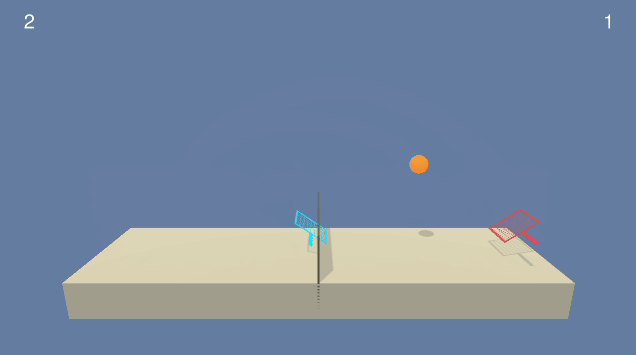
\includegraphics[width=0.75\linewidth]{images/example-env-image.png}
		\caption{A snapshot of the multi-agent Unity-ML tennis environment. The blue racket and red racket agents are tasked to hit the orange ball over the net to the other agent as reliably as possible to keep the ball in play together.}
		\label{fig:example-game-image}
	\end{figure}
	
	\FloatBarrier
	
	Since this is a multi-agent RL environment, there are two agents simultaneously learning from \textit{independent} representations and action computations (i.e., internal policies). Each agent must be able to keep the ball in play for as long as possible, which translates into an episode score that is represented by the \textit{maximum score accumulated by either agent} over that episode. Since this is in effect a somewhat coordinated environment, being able to ensure both agents learn effectively is captured by the goal:
	\begin{itemize}
		\item achieving a 100-episode average max agent score of +0.5.
	\end{itemize}
	
	\section{Approach}
	
	The overall approach used herein was to utilize the \textit{Multi-Agent Deep Deterministic Policy Gradient} (MADDPG) algorithm, which is an extension of the DDPG algorithm to a multi-agent environment. This algorithm is explained in more detail in the following section.
	
	\subsection{MADDPG}
	
	This algorithm is an actor-critic algorithm that adapts Q-learning for a continuous action space, wherein both a Q-function approximation is learned alongside a serially adapted policy. This is similar to the DDPG base algorithm wherein target networks are utilized in learning both an \textit{actor} network and a \textit{critic} network by drawing from experiences in an expanding experience replay buffer. The primary extension of the DDPG algorithm into the multi-agent space is by now training agents using \textit{centralized planning with decentralized execution}. That is, each agent takes in global information about what all agents are experiencing and what actions they take, but each agent has an actor that only leverages its own local information to actually make actions, which is particularly true throughout testing \cite{maddpg}. This helps extend DDPG to multi-agent learning environments in a way that minimizes the non-stationarity that occurs when utilizing DDPG for each agent independently without modification.
	
	Similar to the baseline DDPG algorithm, the \textit{actor} network is responsible for leveraging the approximation of the Q-function to determine an optimal action per time step. This is done by selecting actions as a continuous maxima on the Q and utilize gradient ascent.
	
	\begin{equation}
		\mathop{\mathbb{\text{max}}}_\theta\mathop{\mathbb{E}}_{s\sim D}\left[Q_{\phi}\left(s, \mu_{\theta}(s)\right)\right]
	\end{equation}
	
	Additionally, the \textit{critic} network is only concerned with improving the Q-function approximation, whereby the network evaluates the value of taken actions against the value of predicted actions suggested by the \textit{actor} network. This is remains from the standard DDPG algorithm, and thus follows a valuation from:
	
	\begin{equation}
		Q^*(s_{both}, a_{both}) = \mathop{\mathbb{E}}_{s'_{both} \sim P}\left[r(s_i, a_i) + \gamma\mathop{\mathbb{\text{max}}}_{a'}Q^*(s'_{both}, a'_{both})\right]
	\end{equation}
	for evaluating a Q-function utilizing the Bellman equation for capturing reward and current max estimations on states and actions from the \textit{critic} and \textit{actor} networks. Here, $s_i$ and $a_i$ come from local values an agent observes, whereas $s_{both}$ and $a_{both}$ come from global information of both agents.
	
	Similar to DDPG, noise values are added to the actions of each agent to maintain a level of exploration throughout training, specifically by adding Ornstein-Uhlenbeck noise \cite{ddpg}. During application of the trained models, however, not only are actors now selecting actions using only local information but noise is also removed.
	
	\subsection{Implementation}
	
	The specific implementation of MADDDPG completed in this work largely takes on the same form as the pseudocode in Lowe et al. \cite{maddpg}.
	
	The implementation takes on the following characteristics:
	\begin{itemize}
		\item both \textit{actor} and \textit{critic} networks utilized a baseline and target network pairing during training, where target networks are updated using a per-step soft-update schedule with ratio $\tau$,
		\item the \textit{actor} network seemed to benefit from a simpler architecture in comparison to the \textit{critic} network,
		\item using a repeatable update schedule per step (i.e., the networks can be updated \textit{m} times per step) along with learning rate $\alpha$,
		\item the \textit{critic} for each agent learned from global observation and action information, whereas the \textit{actor} network for each agent only utilized locally available information to that agent.
	\end{itemize}
	
	\FloatBarrier
	
	Using these implementation details on top of the MADDPG algorithm, I settled on the following hyperparameters:
	
	\FloatBarrier
	
	\begin{table}[!ht]
		\centering
		\begin{tabular}{ c | p{6cm} | c }
			\textbf{hyperparameter} & \textbf{utility} & \textbf{value} \\
			\hline
			$\alpha_{actor}$ & \textit{actor} learning rate & $0.001$ \\
			$\alpha_{critic}$ & \textit{critic} learning rate & $0.001$ \\
			$\tau$ & target network soft-update rate & $0.001$ \\
			$\gamma$ & discount factor on future returns & $0.99$ \\
			$t\ update$ & number of steps to take before updating networks & $2$ \\
			$num\ updates$ & number of updates to complete each time networks are updated during training & $5$ \\
			$\mu$ & regression mean for Ornstein-Uhlenbeck noise & $0.0$ \\
			$\theta$ & factor for weighing the delta of value from mean & $0.15$ \\
			$\sigma$ & factor for weighing the Weiner (Gaussian) noise process & $0.2$ \\
			\hline
		\end{tabular}
		\caption{Hyperparameters experimented with to train an agent using MADDPG.}
		\label{tbl:parameters}
	\end{table}
	
	Values were either determined experimentally, such as by varying learning rate $\alpha$, $\tau$, $\gamma$, and the integers for the update schedule, or utilized from the first description of leveraging Ornstein-Uhlenbeck noise in the DDPG algorithm \cite{ddpg} for $\mu$, $\theta$, and $\sigma$.
	
	Lastly, smaller architecture sizes seemed to produce better results for learning, where larger networks tended to show more tendency for residual performance dropoff once solved. Though the smaller networks tended to show this same pattern to some degree, they were able to learn how to consistently hit the ball nearly as well with more stability upon reaching that +0.5 solved average. For a bit more detail on the architectures utilized in these models, they are outlined below in Figure \ref{fig:nn-architecture}.
	
	\FloatBarrier
	
	\begin{figure}[!ht]
		\centering
		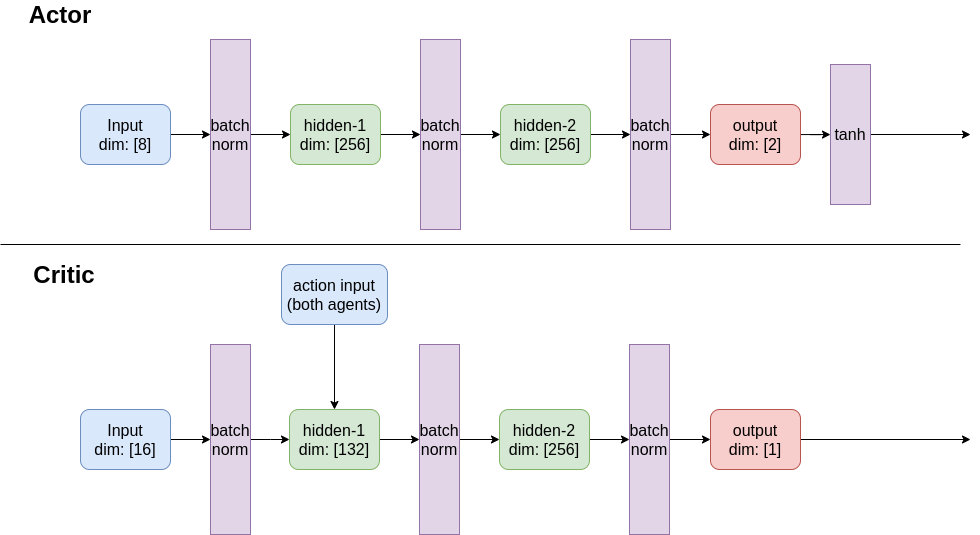
\includegraphics[width=0.75\linewidth]{images/nn_architectures.png}
		\caption{The architectures used in the final \textit{actor} and \textit{critic} networks in the MADDDPG algorithm. Though not specified, all activation functions are ReLU unless otherwise noted. Critic networks utilized global information and thus took in observation and action data from both agents, where actor networks only utilized the observations of an agent itself.}
		\label{fig:nn-architecture}
	\end{figure}
	
	\FloatBarrier
	
	\section{Results and Discussion}
	
	\subsection{Learning Performance}
	
	After determining an optimal set of parameters by running hyperparameter search on $\alpha \in \{0.0001, 0.001, 0.05\}$ for both \textit{actor} and \textit{critic} learning rates, determining stable architectures for hidden layers across both \textit{actor} and \textit{critic} networks, and manually hyperparameter tuning the number of episodes to skip before training and the number of updates per update episode, the following results show training performance over a maximum 4000 episode training session on different major versions of experiments.
	
	\FloatBarrier
	
	\begin{figure}[!ht]
		\centering
		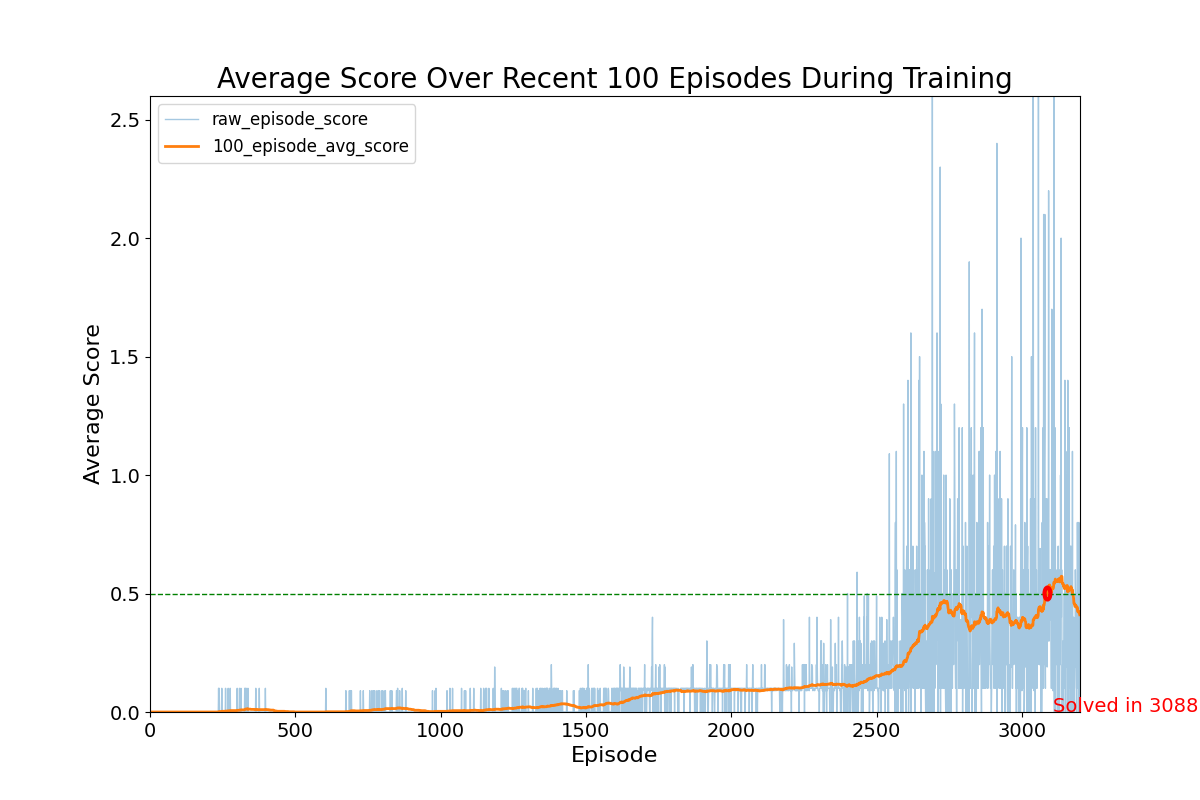
\includegraphics[width=0.75\linewidth]{images/training.png}
		\caption{Per episode and 100-episode average score for episode scores across both agents (max of both agents for an episode). The environment was solved by both agents by achieving a 100-episode average score of +0.5 over 2749 episodes of training.}
		\label{fig:maddpg-results}
	\end{figure}
	
	\FloatBarrier
	
	The results in Figure \ref{fig:maddpg-results} illustrate the ability of the MADDPG algorithm to learn to solve the tennis environment in 2749 episodes when leveraging experiences from both agents for \textit{critic} updates and only local agent information for \textit{actor} updates. After all hyperparameter experimentation and other types of modifications to the algorithm, some improvements that seemed to matter most for achieving more stability in training as shown in Fig. \ref{fig:maddpg-results} were simpler architectures, and maintaining a static Ornstein-Uhlenbeck noise process throughout training (i.e., decaying the noise actually resulted in more variable training).
		
	 Though the agents were able to learn the task well, the stability of learning still left some room for improvement, however, as training proceeded quite rapidly after a certain number of episodes were reached ($\approx$2300 epsiodes). This may be due to the nature of the experience replay buffer cycling out low-reward episodes from early in training. Unclear, however, is why training shows a fair amount of instability around the target episode average of +0.5. Once the agents achieve a score of approximately +0.4, training tends to see more diminishing returns and some regression at times. This may be due to the changes in reward values that the updates to \textit{critic} and even \textit{actor} networks are seeing in later episodes, particularly when there are sporadic high reward episodes (+2.6). Despite these observed patterns, training appears to continue to generally improve throughout. More stable performance above the goal average of +0.5 seems to become more stable towards the end of training as well, around $\approx$3600 episodes. More rigorous hyperparameter tuning and/or experimentation with other multi-agent algorithms may prove for more avenues to show better training performance against the MADDPG results shown herein.
	
	\subsection{Next Steps}
	
	Some obvious next steps were to complete an intended comparison of MADDPG to other multi-agent potential algorithms such as a multi-agent Q-learning agent useful for coordination tasks EAQR \cite{eaqr}. Beyond this, some additional next steps that were thought of to possibly introduce improvement if experimented with appropriately included:
	\begin{itemize}
		\item experimenting with different noise processes, specifically examining how effective an explicit Gaussian noise process would be,
		\item experimenting with different parameters for the Ornstein-Uhlenbeck noise process, particularly for $\theta$ and $\sigma$ for controlling the variance of injected noise,
		\item experimenting with the idea of introducing differences between the \textit{actor} and \textit{critic} network architectures, thereby introducing more fine-tuned abilities of the networks to capitalize on more quickly learning a policy by learning from actions and values somewhat independently, this may be important especially for capturing aspects of learning from global information (i.e., \textit{critic} learning) than only local information,
		\item some level of prioritization and weightings by using a prioritized experience replay buffer \cite{prioritized}, which could help ascertain if issues with stability were in fact due to the nature of experiences sampled from the buffer and how more consistent higher reward experiences affected training stability.
	\end{itemize}
	
	With these potential improvements, there are many avenues to still experiment further with MADDPG before moving on to another algorithm. Improvements that are relevant for DDPG may also be feasible for exploration in this logical extension of DDPG into MADDPG as well.
	
	\section{Conclusion}
	
	With the results shown herein, agents were trained to coordinate their actions to keep a ball passing back and forth for as long as possible using the MADDPG algorithm. This algorithm was able to extend the DDPG algorithm to help agents leverage global information to uncover value, but only act on using local information available to each agent. Though the agents were able to learn the task quite well, there did appear to be some issues with stability as well, and thus show that there are other areas that can be experimented with further to gain some more improved training results.
	
	\bibliographystyle{unsrt}
	\bibliography{refs}
	
\end{document}
